% answers.tex —— 2017 年·全国Ⅱ卷·理科 · 参考答案与详细解析片段
% 由 tools/generate_projects.py 依来源总账自 2017/2017_数学真题_全国2理_试题.md + 2017/2017_数学真题_全国2理_解析正文.md + 2017/2017_数学真题_全国2理_答案要点.md 生成，勿手改（改源 MD 后重跑）


\begin{gknotice}
\textbf{解析归属}：固定来源不附答案。以下推导由本库独立完成并由不同角色盲核，非官方解析。
\end{gknotice}

\begin{answer}
\gksolhead{1}{}

\textbf{题目}：

\(\dfrac{3+i}{1+i}=\)（　）

   (A) \(1+2i\)　　(B) \(1-2i\)　　(C) \(2+i\)　　(D) \(2-i\)

\Needspace{4\baselineskip}
\textbf{解析}

分子分母同乘 \(1-\mathrm i\)，得 \(\dfrac{(3+\mathrm i)(1-\mathrm i)}2=2-\mathrm i\)。

\gkanswer{答案：D（D）}

\end{answer}
\begin{answer}
\gksolhead{2}{}

\textbf{题目}：

设集合 \(A=\{1,2,4\}\)，\(B=\{x\mid x^2-4x+m=0\}\)。若 \(A\cap B=\{1\}\)，则 \(B=\)（　）

   (A) \(\{1,-3\}\)　　(B) \(\{1,0\}\)　　(C) \(\{1,3\}\)　　(D) \(\{1,5\}\)

\Needspace{4\baselineskip}
\textbf{解析}

因 \(1\in A\cap B\)，必有 \(1-4+m=0\)，故 \(m=3\)。方程因式分解为 \((x-1)(x-3)=0\)，其根集为 \(\{1,3\}\)。

\gkanswer{答案：C（D）}

\end{answer}
\begin{answer}
\gksolhead{3}{}

\textbf{题目}：

我国古代数学名著《算法统宗》中有如下问题：“远望巍巍塔七层，红光点点倍加增，共灯三百八十一，请问尖头几盏灯？”意思是：一座 7 层塔共挂了 381 盏灯，且相邻两层中的下一层灯数是上一层灯数的 2 倍，则塔的顶层共有灯（　）

   (A) 1 盏　　(B) 3 盏　　(C) 5 盏　　(D) 9 盏

\Needspace{4\baselineskip}
\textbf{解析}

若顶层有 \(t\) 盏，则七层总数为 \(t(1+2+\cdots+2^6)=127t=381\)，解得 \(t=3\)。

\gkanswer{答案：B（D）}

\end{answer}
\begin{answer}
\gksolhead{4}{}

\textbf{题目}：

如图，网格纸上小正方形的边长为 1，粗实线画出的是某几何体的三视图，该几何体由一平面将一圆柱截去一部分后所得，则该几何体的体积为（　）
\nopagebreak[4]
\begin{center}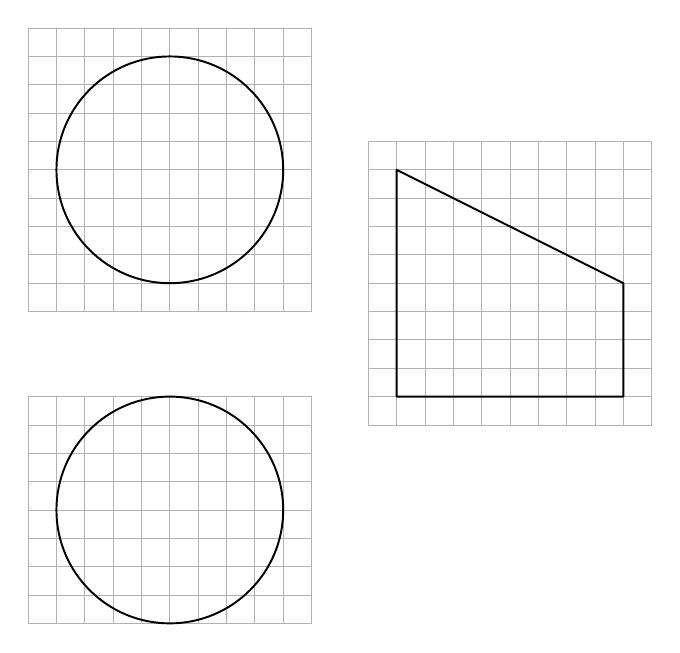
\begin{tikzpicture}[line cap=round,line join=round,line width=0.7pt,scale=0.36]
\begin{scope}[shift={(0,11)}]
  \draw[gray!60,line width=0.3pt] (0,0) grid (10,10);
  \draw (5,5) circle (4);
\end{scope}
\begin{scope}[shift={(12,7)}]
  \draw[gray!60,line width=0.3pt] (0,0) grid (10,10);
  \draw (1,1)--(9,1)--(9,5)--(1,9)--cycle;
\end{scope}
\begin{scope}
  \draw[gray!60,line width=0.3pt] (0,0) grid (10,8);
  \draw (5,4) circle (4);
\end{scope}
\end{tikzpicture}
\end{center}
\nopagebreak[4]
   (A) \(90\pi\)　　(B) \(63\pi\)　　(C) \(42\pi\)　　(D) \(36\pi\)

\Needspace{4\baselineskip}
\textbf{解析}

网格给出底面半径 \(3\)，截切后圆柱轴向两侧的端高为 \(10\) 与 \(4\)。斜平面高度在圆盘上作线性变化，平均高度为 \(7\)，体积为 \(\pi\cdot3^2\cdot7\)。

\gkanswer{答案：B（D）}

\end{answer}
\begin{answer}
\gksolhead{5}{}

\textbf{题目}：

\Needspace{5\baselineskip}
设 \(x,y\) 满足约束条件
\nopagebreak[4]
   \[
   \begin{cases}
   2x+3y-3\leq 0,\\
   2x-3y+3\geq 0,\\
   y+3\geq 0,
   \end{cases}
   \]
   则 \(z=2x+y\) 的最小值是（　）

   (A) \(-15\)　　(B) \(-9\)　　(C) \(1\)　　(D) \(9\)

\Needspace{4\baselineskip}
\textbf{解析}

可行域的最低点由 \(y=-3\) 与 \(2x-3y+3=0\) 相交得到 \((-6,-3)\)，目标值为 \(-15\)。检查其余边界顶点的目标值均较大，故最小值在该点取得。

\gkanswer{答案：A（D）}

\end{answer}
\begin{answer}
\gksolhead{6}{}

\textbf{题目}：

安排 3 名志愿者完成 4 项工作，每人至少完成 1 项，每项工作由 1 人完成，则不同的安排方式共有（　）

   (A) 12 种　　(B) 18 种　　(C) 24 种　　(D) 36 种

\Needspace{4\baselineskip}
\textbf{解析}

四项工作分给三人且无人空缺，人数分配必为 \((2,1,1)\)。选出由同一人完成的两项，再把三组非空工作分配给三名不同志愿者，共 \(\binom42\cdot3!=36\) 种。

\gkanswer{答案：D（D）}

\end{answer}
\begin{answer}
\gksolhead{7}{}

\textbf{题目}：

甲、乙、丙、丁四位同学一起去向老师询问成语竞赛的成绩。老师说：你们四人中有 2 位优秀，2 位良好，我现在给甲看乙、丙的成绩，给乙看丙的成绩，给丁看甲的成绩。看后甲对大家说：我还是不知道我的成绩。根据以上信息，则（　）

   (A) 乙可以知道四人的成绩　　(B) 丁可以知道四人的成绩

   (C) 乙、丁可以知道对方的成绩　　(D) 乙、丁可以知道自己的成绩

\Needspace{4\baselineskip}
\textbf{解析}

甲看乙、丙后仍不能确定自己，说明乙、丙一优一良；否则甲可由总人数配额直接推出自己的成绩。于是甲、丁也一优一良，乙看丙、丁看甲后都能确定自身成绩。

\gkanswer{答案：D（D）}

\end{answer}
\begin{answer}
\gksolhead{8}{}

\textbf{题目}：

执行如图的程序框图，如果输入的 \(a=-1\)，则输出的 \(S=\)（　）
\nopagebreak[4]
\begin{center}\begin{tikzpicture}[line width=0.75pt,line cap=round,line join=round,font=\small]
\node[draw,rounded corners,minimum width=1.35cm,minimum height=0.5cm] (start) at (0,0) {开始};
\node[draw,minimum width=2.2cm,minimum height=0.55cm] (input) at (0,-0.95) {输入 $a$};
\node[draw,minimum width=2.7cm,minimum height=0.55cm] (init) at (0,-1.9) {$S=0,\ K=1$};
\coordinate (dt) at (0,-2.6);
\coordinate (dr) at (1.9,-3.2);
\coordinate (db) at (0,-3.8);
\coordinate (dl) at (-1.9,-3.2);
\draw (dt)--(dr)--(db)--(dl)--cycle;
\node at (0,-3.2) {$K\le 6$};
\node[draw,minimum width=3.0cm,minimum height=0.55cm] (sum) at (0,-4.55) {$S=S+a\cdot K$};
\node[draw,minimum width=2.3cm,minimum height=0.55cm] (flip) at (0,-5.45) {$a=-a$};
\node[draw,minimum width=2.6cm,minimum height=0.55cm] (next) at (0,-6.35) {$K=K+1$};
\node[draw,minimum width=1.9cm,minimum height=0.55cm] (out) at (3.6,-3.2) {输出 $S$};
\node[draw,rounded corners,minimum width=1.35cm,minimum height=0.5cm] (end) at (3.6,-4.2) {结束};
\draw[->] (start)--(input);
\draw[->] (input)--(init);
\draw[->] (init)--(dt);
\draw[->] (db)--node[right]{是}(sum);
\draw[->] (sum)--(flip);
\draw[->] (flip)--(next);
\draw[->] (next.west)--(-2.65,-6.35)--(-2.65,-3.2)--(dl);
\draw[->] (dr)--node[above]{否}(out.west);
\draw[->] (out)--(end);
\end{tikzpicture}
\end{center}
\nopagebreak[4]
   (A) 2　　(B) 3　　(C) 4　　(D) 5

\Needspace{4\baselineskip}
\textbf{解析}

根据流程图，\(K\) 从 1 依次取到 6，且每轮先累加 \(aK\) 再令 \(a\) 变号。因此总和为 \(-1+2-3+4-5+6\)。

\gkanswer{答案：B（D）}

\end{answer}
\begin{answer}
\gksolhead{9}{}

\textbf{题目}：

若双曲线 \(C:\dfrac{x^2}{a^2}-\dfrac{y^2}{b^2}=1\)（\(a>0,b>0\)）的一条渐近线被圆 \((x-2)^2+y^2=4\) 所截得的弦长为 2，则 \(C\) 的离心率为（　）

   (A) \(2\)　　(B) \(\sqrt{3}\)　　(C) \(\sqrt{2}\)　　(D) \(\dfrac{2\sqrt{3}}{3}\)

\Needspace{4\baselineskip}
\textbf{解析}

圆半径为 \(2\)，弦长为 \(2\)，故圆心到渐近线的距离为 \(\sqrt{2^2-1^2}=\sqrt3\)。设渐近线斜率绝对值 \(m=b/a\)，则 \(2m/\sqrt{1+m^2}=\sqrt3\)，得 \(b^2/a^2=3\)，再由 \(e^2=1+b^2/a^2\) 求离心率。

\gkanswer{答案：A（D）}

\end{answer}
\begin{answer}
\gksolhead{10}{}

\textbf{题目}：

已知直三棱柱 \(ABC-A_1B_1C_1\) 中，\(\angle ABC=120^\circ\)，\(AB=2\)，\(BC=CC_1=1\)，则异面直线 \(AB_1\) 与 \(BC_1\) 所成角的余弦值为（　）

   (A) \(\dfrac{\sqrt{3}}{2}\)　　(B) \(\dfrac{\sqrt{15}}{5}\)　　(C) \(\dfrac{\sqrt{10}}{5}\)　　(D) \(\dfrac{\sqrt{3}}{3}\)

\Needspace{4\baselineskip}
\textbf{解析}

取 \(B=(0,0,0),C=(1,0,0),A=(-1,\sqrt3,0)\)，并令棱柱高沿 \(z\) 轴。方向向量可取 \(\overrightarrow{AB_1}=(1,-\sqrt3,1)\)、\(\overrightarrow{BC_1}=(1,0,1)\)，内积为 \(2\)，模长乘积为 \(\sqrt{10}\)。

\gkanswer{答案：C（D）}

\end{answer}
\begin{answer}
\gksolhead{11}{}

\textbf{题目}：

若 \(x=-2\) 是函数 \(f(x)=(x^2+ax-1)e^{x-1}\) 的极值点，则 \(f(x)\) 的极小值为（　）

   (A) \(-1\)　　(B) \(-2e^{-3}\)　　(C) \(5e^{-3}\)　　(D) \(1\)

\Needspace{4\baselineskip}
\textbf{解析}

求导并代入极值点 \(x=-2\)，由驻点条件得 \(a=-1\)。此时导数可因式分解为 \(e^{x-1}(x+2)(x-1)\)，在 \(x=1\) 处由负变正，故该处取极小值。

\gkanswer{答案：A（D）}

\end{answer}
\begin{answer}
\gksolhead{12}{}

\textbf{题目}：

已知 \(\triangle ABC\) 是边长为 2 的等边三角形，\(P\) 为平面 \(ABC\) 内一点，则 \(\overrightarrow{PA}\cdot(\overrightarrow{PB}+\overrightarrow{PC})\) 的最小值是（　）

   (A) \(-2\)　　(B) \(-\dfrac{3}{2}\)　　(C) \(-\dfrac{4}{3}\)　　(D) \(-1\)

\Needspace{4\baselineskip}
\textbf{解析}

\Needspace{5\baselineskip}
以等边三角形中心为原点，令顶点位置向量为 \(\mathbf a,\mathbf b,\mathbf c\)，有 \(\mathbf a+\mathbf b+\mathbf c=0\) 且 \(|\mathbf a|^2=4/3\)。目标式配方为
\nopagebreak[4]
\[
2\left|\mathbf p-\frac{\mathbf a}{4}\right|^2-\frac98|\mathbf a|^2,
\]
其平方项可取零且点 \(\mathbf a/4\) 在三角形内。

\gkanswer{答案：B（D）}

\end{answer}
\begin{answer}
\gksolhead{13}{}

\textbf{题目}：

一批产品的二等品率为 0.02，从这批产品中每次随机取一件，有放回地抽取 100 次，\(X\) 表示抽到的二等品件数，则 \(DX=\)\gkblank{}。

\Needspace{4\baselineskip}
\textbf{解析}

二项分布方差为 \(np(1-p)\)，代入 \(n=100,p=0.02\) 得 \(1.96\)。

\gkanswer{答案：\(1.96\)（D）}

\end{answer}
\begin{answer}
\gksolhead{14}{}

\textbf{题目}：

函数 \(f(x)=\sin^2x+\sqrt{3}\cos x-\dfrac{3}{4}\)（\(x\in[0,\dfrac{\pi}{2})\)）的最大值是\gkblank{}。

\Needspace{4\baselineskip}
\textbf{解析}

令 \(t=\cos x\in(0,1]\)，原式化为 \(\frac14-t^2+\sqrt3t=1-(t-\sqrt3/2)^2\)。顶点落在取值范围内。

\gkanswer{答案：\(1\)（D）}

\end{answer}
\begin{answer}
\gksolhead{15}{}

\textbf{题目}：

等差数列 \(\{a_n\}\) 的前 \(n\) 项和为 \(S_n\)，\(a_3=3\)，\(S_4=10\)，则 \(\displaystyle\sum_{k=1}^{n}\dfrac{1}{S_k}=\)\gkblank{}。

\Needspace{4\baselineskip}
\textbf{解析}

由 \(a_1+2d=3\)、\(2a_1+3d=5\) 得首项与公差均为 1，于是 \(S_k=k(k+1)/2\)。利用 \(2/[k(k+1)]=2(1/k-1/(k+1))\) 后作望远镜求和。

\gkanswer{答案：\(\dfrac{2n}{n+1}\)（D）}

\end{answer}
\begin{answer}
\gksolhead{16}{}

\textbf{题目}：

已知 \(F\) 是抛物线 \(C:y^2=8x\) 的焦点，\(M\) 是 \(C\) 上一点，\(FM\) 的延长线交 \(y\) 轴于点 \(N\)。若 \(M\) 为 \(FN\) 的中点，则 \(|FN|=\)\gkblank{}。

\Needspace{4\baselineskip}
\textbf{解析}

焦点为 \(F=(2,0)\)。设 \(N=(0,t)\)，中点条件给 \(M=(1,t/2)\)。代入抛物线得 \(t^2/4=8\)，再由两点距离计算 \(|FN|\)。

\gkanswer{答案：\(6\)（D）}

\end{answer}
\begin{answer}
\gksolhead{17}{}

\textbf{题目}：

\(\triangle ABC\) 的内角 \(A,B,C\) 的对边分别为 \(a,b,c\)，已知 \(\sin(A+C)=8\sin^2\dfrac{B}{2}\)。

   (1) 求 \(\cos B\)；

   (2) 若 \(a+c=6\)，\(\triangle ABC\) 面积为 2，求 \(b\)。

\Needspace{4\baselineskip}
\textbf{解析}

\gksubpart{(1) 角与边}

因 \(A+C=\pi-B\)，题设化为 \(\sin B=8\sin^2(B/2)\)。用半角公式约去正数 \(\sin(B/2)\)，得 \(\tan(B/2)=1/4\)，从而 \(\sin B=8/17,\cos B=15/17\)。

\gksubpart{(2) 余弦定理}

\Needspace{5\baselineskip}
面积条件与 \(\sin B=8/17\) 给出 \(ac=17/2\)。又 \(a+c=6\)，故
\nopagebreak[4]
\[
b^2=(a+c)^2-2ac(1+\cos B)=36-17\cdot\frac{32}{17}=4.
\]

\gkanswer{答案（1）：\(\cos B=\dfrac{15}{17}\)（D）}

\gkanswer{答案（2）：\(b=2\)（D）}

\end{answer}
\begin{answer}
\gksolhead{18}{}

\textbf{题目}：

海水养殖场进行某水产品的新、旧网箱养殖方法的产量对比，收获时各随机抽取了 100 个网箱，测量各箱水产品的产量（单位：kg），其频率分布直方图如图：
\nopagebreak[4]
\begin{center}\begin{tikzpicture}[x=0.68cm,y=0.68cm,line width=0.55pt,font=\scriptsize]
\begin{scope}
  \draw[->] (0,0)--(9.45,0);
  \draw[->] (0,0)--(0,7.55);
  \foreach \y/\lab/\x in {1.2/0.012/0,1.4/0.014/-1,2.0/0.020/0,2.4/0.024/0,3.2/0.032/0,3.4/0.034/-1,4.0/0.040/0} {
    \draw[densely dashed,gray] (0,\y)--(9,\y);
    \node[left] at (\x,\y) {\lab};
  }
  \foreach \x/\lab in {0/25,1/30,2/35,3/40,4/45,5/50,6/55,7/60,8/65,9/70} {
    \draw (\x,0)--(\x,-0.08);
    \node[below] at (\x,-0.12) {\lab};
  }
  \foreach \x/\h in {0/1.2,1/1.4,2/2.4,3/3.4,4/4.0,5/3.2,6/2.0,7/1.2,8/1.2} {
    \draw[fill=white] (\x,0) rectangle ++(1,\h);
  }
  \node[anchor=west] at (0.18,7.15) {频率/组距};
  \node at (4.5,-0.9) {箱产量/kg};
  \node at (4.5,-1.55) {旧养殖法};
\end{scope}
\begin{scope}[shift={(12,0)}]
  \draw[->] (0,0)--(7.45,0);
  \draw[->] (0,0)--(0,7.55);
  \foreach \y/\lab/\x in {0.4/0.004/0,0.8/0.008/-1,1.0/0.010/0,2.0/0.020/0,4.4/0.044/0,4.6/0.046/-1,6.8/0.068/0} {
    \draw[densely dashed,gray] (0,\y)--(7,\y);
    \node[left] at (\x,\y) {\lab};
  }
  \foreach \x/\lab in {0/35,1/40,2/45,3/50,4/55,5/60,6/65,7/70} {
    \draw (\x,0)--(\x,-0.08);
    \node[below] at (\x,-0.12) {\lab};
  }
  \foreach \x/\h in {0/0.4,1/2.0,2/4.4,3/6.8,4/4.6,5/1.0,6/0.8} {
    \draw[fill=white] (\x,0) rectangle ++(1,\h);
  }
  \node[anchor=west] at (0.18,7.15) {频率/组距};
  \node at (3.5,-0.9) {箱产量/kg};
  \node at (3.5,-1.55) {新养殖法};
\end{scope}
\end{tikzpicture}
\end{center}
\nopagebreak[4]
   (1) 设两种养殖方法的箱产量相互独立，记 \(A\) 表示事件“旧养殖法的箱产量低于 50 kg，新养殖法的箱产量不低于 50 kg”，估计 \(A\) 的概率；

   (2) 填写下面列联表，并根据列联表判断是否有 99\% 的把握认为箱产量与养殖方法有关；

\begin{center}
\begin{tabular}{lrr}
\toprule
 & 箱产量 < 50 kg & 箱产量 $\geq$ 50 kg \\
\midrule
旧养殖法 &  &  \\
新养殖法 &  &  \\
\bottomrule
\end{tabular}
\end{center}

   (3) 根据箱产量的频率分布直方图，求新养殖法箱产量的中位数的估计值（精确到 0.01）。

\Needspace{10\baselineskip}
   附：

\begin{center}
\begin{tabular}{lrrr}
\toprule
\(P(K^2\geq k)\) & 0.050 & 0.010 & 0.001 \\
\midrule
\(K\) & 3.841 & 6.635 & 10.828 \\
\bottomrule
\end{tabular}
\end{center}

\nopagebreak[4]
   \[
   K^2=\frac{n(ad-bc)^2}{(a+b)(c+d)(a+c)(b+d)}.
   \]

\Needspace{4\baselineskip}
\textbf{解析}

\gksubpart{(1) 独立事件概率}

\Needspace{5\baselineskip}
组距为 \(5\,\mathrm{kg}\)。旧法低于 \(50\,\mathrm{kg}\) 的频率为
\nopagebreak[4]
\[
5(0.012+0.014+0.024+0.034+0.040)=0.62,
\]
新法不低于 \(50\,\mathrm{kg}\) 的频率为 \(5(0.068+0.046+0.010+0.008)=0.66\)。按两次随机抽取相互独立相乘。

\gksubpart{(2) 独立性检验}

\Needspace{5\baselineskip}
两组各抽取 \(100\) 个网箱，列联表计数为旧法 \((62,38)\)、新法 \((34,66)\)。代入原题公式得到
\nopagebreak[4]
\[
K^2=\frac{200(62\cdot66-38\cdot34)^2}{100\cdot100\cdot96\cdot104}=\frac{1225}{78}\approx15.705,
\]
超过 99\% 水平的临界值 \(6.635\)。

\gksubpart{(3) 中位数估计}

新法低于 \(50\,\mathrm{kg}\) 的累计频率为 \(0.34\)，所以中位数落在 \([50,55)\) 组。该组频率密度为 \(0.068\)，按组内均匀插值，估计值为 \(50+(0.50-0.34)/0.068\)。

\gkanswer{答案（1）：\(P(A)=0.4092\)（D）}

\gkanswer{答案（2）：列联表为旧法 \((62,38)\)、新法 \((34,66)\)；\(K^2=\dfrac{1225}{78}\approx15.705>6.635\)，有 99\% 的把握认为产量与方法有关（D）}

\gkanswer{答案（3）：新法估计中位数约为 \(52.35\,\mathrm{kg}\)（D）}

\end{answer}
\begin{answer}
\gksolhead{19}{}

\textbf{题目}：

如图，在四棱锥 \(P-ABCD\) 中，侧面 \(PAD\) 为等边三角形且垂直于底面 \(ABCD\)，\(AB=BC=\dfrac{1}{2}AD\)，\(\angle BAD=\angle ABC=90^\circ\)，\(E\) 是 \(PD\) 的中点。
\nopagebreak[4]
\begin{center}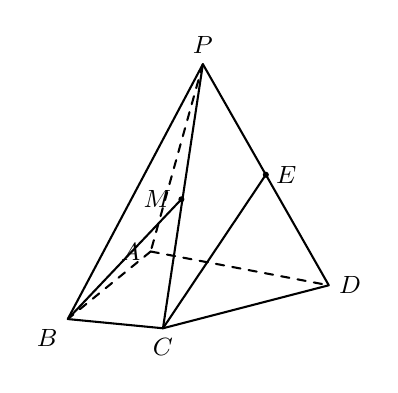
\begin{tikzpicture}[x=0.78cm,y=0.78cm,line cap=round,line join=round,line width=0.75pt,font=\small]
\coordinate (A) at (1.35,1.1);
\coordinate (B) at (0,0);
\coordinate (C) at (1.55,-0.15);
\coordinate (D) at (4.25,0.55);
\coordinate (P) at (2.2,4.15);
\coordinate (M) at (1.85,1.95);
\coordinate (E) at (3.225,2.35);
\draw (P)--(B)--(C)--(D)--(P);
\draw (P)--(C);
\draw[dashed] (P)--(A);
\draw[dashed] (A)--(B);
\draw[dashed] (A)--(D);
\draw (B)--(M);
\draw (C)--(E);
\fill (M) circle (1.1pt);
\fill (E) circle (1.1pt);
\node[above] at (P) {$P$};
\node[below left] at (B) {$B$};
\node[below] at (C) {$C$};
\node[right] at (D) {$D$};
\node[left] at (A) {$A$};
\node[left] at (M) {$M$};
\node[right] at (E) {$E$};
\end{tikzpicture}
\end{center}
\nopagebreak[4]
   (1) 证明：直线 \(CE\parallel\) 平面 \(PAB\)；

   (2) 点 \(M\) 在棱 \(PC\) 上，且直线 \(BM\) 与底面 \(ABCD\) 所成角为 \(45^\circ\)，求二面角 \(M-AB-D\) 的余弦值。

\Needspace{4\baselineskip}
\textbf{解析}

\gksubpart{(1) 线面平行}

令 \(AB=BC=1,AD=2\)，取 \(A=(0,0,0),B=(0,1,0),C=(1,1,0),D=(2,0,0),P=(1,0,\sqrt3)\)，由中点条件得 \(E=(3/2,0,\sqrt3/2)\)。向量 \(\overrightarrow{CE}\) 可写为平面 \(PAB\) 内两方向向量的线性组合，故其平行于该平面。

\gksubpart{(2) 二面角}

令 \(M=P+t(C-P)\)。由 \(BM\) 与底面夹角为 \(45^\circ\)，比较竖直分量与水平投影长度得 \(1-t=1/\sqrt2\)。在垂直于 \(AB\) 的截面中取两平面方向向量，化为平面向量夹角后其余弦为 \(\sqrt{2/5}=\sqrt{10}/5\)。

\gkanswer{答案（1）：\(CE\parallel\) 平面 \(PAB\)（D）}

\gkanswer{答案（2）：二面角余弦为 \(\dfrac{\sqrt{10}}5\)（D）}

\end{answer}
\begin{answer}
\gksolhead{20}{}

\textbf{题目}：

设 \(O\) 为坐标原点，动点 \(M\) 在椭圆 \(C:\dfrac{x^2}{2}+y^2=1\) 上，过 \(M\) 作 \(x\) 轴的垂线，垂足为 \(N\)，点 \(P\) 满足 \(\overrightarrow{NP}=\sqrt{2}\,\overrightarrow{NM}\)。

   (1) 求点 \(P\) 的轨迹方程；

   (2) 设点 \(Q\) 在直线 \(x=-3\) 上，且 \(\overrightarrow{OP}\cdot\overrightarrow{PQ}=1\)。证明：过点 \(P\) 且垂直于 \(OQ\) 的直线 \(l\) 过 \(C\) 的左焦点 \(F\)。

\Needspace{4\baselineskip}
\textbf{解析}

\gksubpart{(1) 轨迹}

设 \(M=(u,v)\)，则 \(N=(u,0)\) 且 \(P=(u,\sqrt2v)\)。由椭圆关系 \(u^2/2+v^2=1\) 得 \(P\) 满足 \(x^2+y^2=2\)。

\gksubpart{(2) 焦点与垂直关系}

\Needspace{5\baselineskip}
记 \(P=(x,y),Q=(-3,t)\)。点积条件与 \(x^2+y^2=2\) 合并为 \(yt=3(x+1)\)。因此
\nopagebreak[4]
\[
\overrightarrow{OQ}\cdot\overrightarrow{PF}=(-3,t)\cdot(-1-x,-y)=3(x+1)-ty=0,
\]
其中 \(F=(-1,0)\) 为椭圆左焦点。

\gkanswer{答案（1）：点 \(P\) 的轨迹为 \(x^2+y^2=2\)（D）}

\gkanswer{答案（2）：过 \(P\) 且垂直于 \(OQ\) 的直线经过椭圆左焦点 \(F=(-1,0)\)（D）}

\end{answer}
\begin{answer}
\gksolhead{21}{}

\textbf{题目}：

已知函数 \(f(x)=ax^2-ax-x\ln x\)，且 \(f(x)\geq 0\)。

   (1) 求 \(a\)；

   (2) 证明：\(f(x)\) 存在唯一的极大值点 \(x_0\)，且 \(e^{-2}<f(x_0)<2^{-2}\)。

\Needspace{4\baselineskip}
\textbf{解析}

\gksubpart{(1) 参数}

定义域为 \(x>0\)。由 \(f(1)=0\) 及处处非负，内点 \(x=1\) 必为极小值点，故 \(f'(1)=a-1=0\)。取 \(a=1\) 后，\(f(x)=x(x-1-\ln x)\ge0\)，与对数不等式一致。

\gksubpart{(2) 极大值点与函数值界}

令 \(h(x)=f'(x)=2x-2-\ln x\)，则 \(h'(x)=2-1/x\)。在 \((0,1/2)\) 上 \(h\) 严格递减，从 \(+\infty\) 降至 \(\ln2-1<0\)，有唯一零点 \(x_0\)；在 \((1/2,+\infty)\) 严格递增且在 1 处为零。由导数符号得 \(x_0\) 为唯一极大值点。方程 \(h(x_0)=0\) 化为 \(\ln x_0=2x_0-2\)，从而 \(f(x_0)=x_0(1-x_0)\)。利用 \(0<x_0<1/2\) 与 \(2x+\ln(1-x)>0\)（\(0<x<1/2\)）夹出题设的严格上下界。

\gkanswer{答案（1）：\(a=1\)（D）}

\gkanswer{答案（2）：唯一极大值点 \(x_0\in(0,\tfrac12)\)，且 \(e^{-2}<f(x_0)<\tfrac14\)（D）}

\end{answer}
\begin{answer}
\gksolhead{22}{}

\textbf{题目}：

在直角坐标系 \(xOy\) 中，以坐标原点为极点，\(x\) 轴的正半轴为极轴建立极坐标系，曲线 \(C_1\) 的极坐标方程为 \(\rho\cos\theta=4\)。

   (1) \(M\) 为曲线 \(C_1\) 上的动点，点 \(P\) 在线段 \(OM\) 上，且满足 \(|OM|\cdot|OP|=16\)，求点 \(P\) 的轨迹 \(C_2\) 的直角坐标方程；

   (2) 设点 \(A\) 的极坐标为 \((2,\dfrac{\pi}{3})\)，点 \(B\) 在曲线 \(C_2\) 上，求 \(\triangle OAB\) 面积的最大值。

\Needspace{4\baselineskip}
\textbf{解析}

\gksubpart{(1) 轨迹}

设 \(M=(4,t)\)，并令 \(P=\lambda M\)。距离乘积条件给 \(\lambda=16/(16+t^2)\)，故消参得到 \(x^2+y^2=4x\)。有限参数对应 \(x>0\)，原点仅是极限点而不在实际轨迹上。

\gksubpart{(2) 面积}

点 \(A=(1,\sqrt3)\)，而圆心 \((2,0)\)、半径 2 的轨迹圆上点为 \(B\)。面积由 \(|\det(A,B)|/2\) 给出；行列式在圆心处的常量项与沿半径方向变化量分别为 \(2\sqrt3\)、\(4\)，且达到极值的点不是原点。

\gkanswer{答案（1）：\(x^2+y^2=4x\)，实际轨迹不含原点（即再要求 \(x>0\)）（D）}

\gkanswer{答案（2）：三角形面积最大值为 \(2+\sqrt3\)（D）}

\end{answer}
\begin{answer}
\gksolhead{23}{}

\textbf{题目}：

已知 \(a>0,b>0,a^3+b^3=2\)，证明：

   (1) \((a+b)(a^5+b^5)\geq 4\)；

   (2) \(a+b\leq 2\)。

\Needspace{4\baselineskip}
\textbf{解析}

\gksubpart{(1) 幂不等式}

由柯西不等式，\((a+b)(a^5+b^5)\ge(a^3+b^3)^2=4\)。

\gksubpart{(2) 和的上界}

幂平均不等式给 \((a+b)/2\le((a^3+b^3)/2)^{1/3}=1\)，故所需上界成立；两部分在 \(a=b=1\) 时取等号。

\gkanswer{答案（1）：\((a+b)(a^5+b^5)\ge4\)（D）}

\gkanswer{答案（2）：\(a+b\le2\)（D）}

\end{answer}